\Chapter{Processz ütemezés}

\Section{Az ütemezési probléma}

\Section{Elterjedt ütemezési stratégiák}

\SubSection{$\mathcal{O}(n)$}
Az $O(n)$ ütemező, amelyet a Linux kernelben használtak 2.4 és 2.6 verziók között. A müködési elve egyszerűnek mondható, mivel végigiterál az összes futtatható processzen, kiszámolja a prioritásaikat, majd a "legjobbat" választja meg futásra. A "legjobb" jelző, a processzekhez rendelt nice értékből és a felhasználatlan időszeletből kalkulálódik.
Ez egy $O(n)$ műveletigényű algoritmus volt, ahol az $n$ a futtatható processzek számát jelölte. Emiatt nagy processzámnál nem volt elég effektív és a valós idejű processzek így kiszámíthatlanok lettek.
%TODO http://www.cse.iitm.ac.in/~chester/courses/16o_os/slides/7_Scheduling.pdf
\SubSection{$\mathcal{O}(1)$}
Az $O(1)$ ütemezőt Linux kernel 2.6-os verziótól 2.6.22 ig használták. Konstans idő alatt választott következő processzt futásra, emiatt nagy processz szám mellett is használható volt, az $O(n)$-es ütemezővel ellentétben.
A processzeket két részre osztja, típus szerint. A valós idejű processzek 0-99-ig kaptak prioritás szinteket, amíg a normál processzek(Batch vagy inveractive) 100-139-ig. Itt a 100-as prioritás jelöli a legfontosabb processzt, amíg a 139 a legkevésbé fontosat. Normál processzekhez egy alapértelmezett 120-as statikus prioritást rendeltek. A nice paranccsal tudjuk ezt az alapértelmezett prioritást változtatni.
%TODO http://www.cse.iitm.ac.in/~chester/courses/16o_os/slides/7_Scheduling.pdf
%TODO https://www.researchgate.net/publication/4376448_Fairness_and_interactive_performance_of_O1_and_CFS_Linux_kernel_schedulers
\begin{python}
$ nice -n N ./a.out 
\end{python}
%$
Ahol az N értéke +19 és -20 között mozoghat.

Normál processzek ütemezésénél, processzoronként, két listát tart nyilván amiben tárolódnak a futásra kész processzek. (Active run queue, Expired run queue)
Mindig az aktív listából választja a legfontosabb processzt, futásra. Amikor végzett, a futó processz átkerül az expired run queue-ba, egy új dinamikusan számolt prioritással.
Emiatt ahogy haladunk előre az időben az active run queue-ból folyamatosan fogynak el a processzek.  Amikor az active run queue végzett a processzekkel, a két lista felcserélődik és folyatatódik a végrehajtás az új listával.
Annak érdekében hogy meglehessen különböztetni a batch és az interactive processzeket, egy úgynevezett "bonus" valtozot tartunk nyilván, ami dinamikus prioritás számításnál fog előkerülni. Ennek az értéke 0 és 10 között mozoghat.
\begin{cpp}
dynamic priority = MAX(100, MIN(static priority - bonus + 5), 139)) 
\end{cpp}
Amikor a bonus változó értéke kisebb mint 5, arra utal hogy kevesebb interakciót fog végezni a felhasználóval, így több cpu lázas szakasza lesz a processznek élete során. Konvergálódik a 139-es prioritás felé, ezt a processz típust nevezzük batch processznek.(Kevésbé lesz fontos) 
Ha a bonus változó értéke több mint 5 lesz, valószínűleg a processz élete során sok interakcióra lesz szüksége a felhasználóval, tehát ez egy interactive processz (másnéven I/O lázas). A prioritása konvergálódik a 100 felé. Az interactive processzek általában nem fejezik be az időszeletüket amit kapnak, ezért nekik nagyobb időszeletet kell hogy adjunk. Így bizonyosodhatunk meg arról hogy ténylegesen be tudja fejezni az instrukció sorozatot, és majd ha kész, lemond önszántából a CPU-ról.

Az időszelet meghatározása úgy történik, hogy amelyik processz kevesebb mint 120-as prioritással rendelkezik, nagyobb időszeletet kap, 120-nál nagyobb prioritású processzek pedig kevesebbet.
\begin{cpp}
if priority < 120 
	time slice = (140 - priority) * 20    milliseconds 
else
	time slice = (140 - priority) * 5   milliseconds 
\end{cpp}

\begin{figure}[h]
\centering
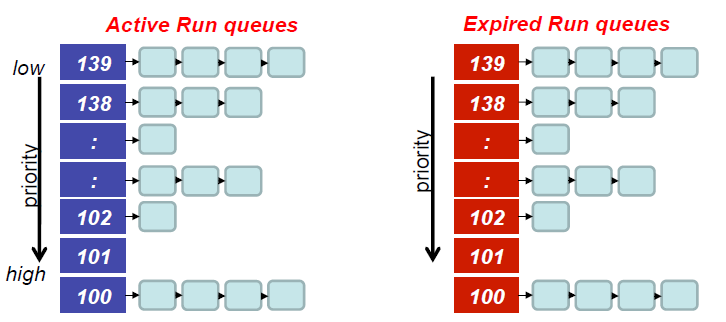
\includegraphics[width=\textwidth]{images/activeexpiredrunqueue.png}
\caption{Active and Expired Run queues}
%TODO átrajzolni

\label{fig:Active and expired runqueues}
\end{figure}

\SubSection{Completely Fair Scheduler}
A "Completely Fair Scheduler", azaz (CFS) ütemezőt még Molnár Ingo mutatta be 2007 júliusában, amit Linus Torvalds be is olvasztott a Linux kernel(2.6.23) rendszermagjába. A korábbi $\mathcal{O}(1)$ ütemező komponenseit, mint például: az aktív és lejárt folyamatok tömbje, interaktív processzek azonosítása, prioritás alapú időszelet koncepció, eltávolították, a hatékonyság javíásának érdekében. 
%TODO http://www.cse.iitm.ac.in/~chester/courses/16o_os/slides/7_Scheduling.pdf
%TODO https://scslab-intern.gitbooks.io/linux-kernel-hacking/content/chapter04.html
%TODO https://elixir.bootlin.com/linux/v5.8.5/source/kernel/sched/fair.c
%TODO https://www.researchgate.net/publication/4376448_Fairness_and_interactive_performance_of_O1_and_CFS_Linux_kernel_schedulers
Az alapvető adatstruktúra az ütemezőben a folyamatok Run-queue. A run-queue-t a \textit{kernel/sched.h}-ben definiálták, mint \textit{struct rq}. Maga a run-queue egy lista ami a futtatható entitásokat tartalmazza, minden processzorhoz tartozik egy run-queue. A run-queue-nak, különböző területei vannak mint például cfs, real time, deadline run queue-k.
Mindegyiknek megvan a saját ütemezője.
\begin{cpp}
struct rq {
      struct cfs_rq cfs;  // completely fair scheduler
      struct rt_rq rt;    // real-time scheduler
      struct dl_rq dl;    // deadline scheduler
}
\end{cpp}

%\begin{figure}[h!]
%\centering
%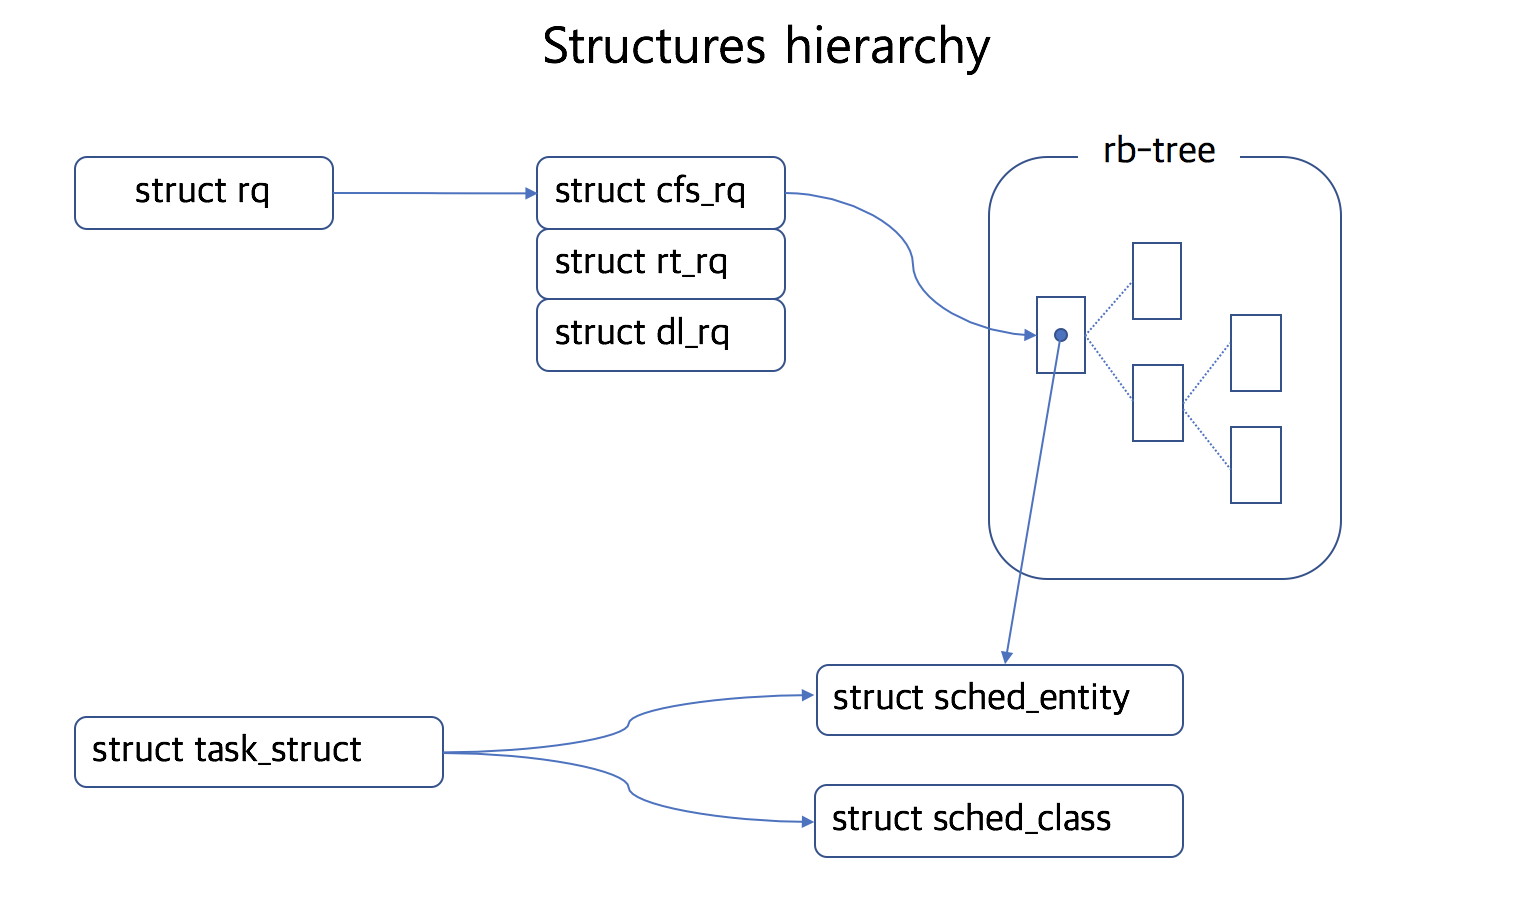
\includegraphics[width=\textwidth]{images/structures.png}
%\caption{Struktúra hierarchia}
%\label{fig:structurehierarchi}
%\end{figure}
Az ideális ütemezés érdekében, a CFS algoritmus felosztja a processzor időszeletet a processzek között és minden processz $(100/N)\%$ részt kap meg, ahol az $N$ a processzek számát jelöli.
\begin{table}[h]
\centering
\caption{A processz végrehajtásához szükséges idő}
\label{tab:processtimes}
\begin{tabular}{|c|c|}
\hline
Processz & idő \\
\hline
A & 8ms \\
B & 4ms \\
C & 16ms \\
D & 4ms \\
\hline
\end{tabular}
\end{table}

\begin{table}[h]
\centering
\caption{A processzekre jutó időszeletek}
\label{tab:timeslices}
\begin{tabular}{|c|c|c|c|c|c|c|c|c|}
\hline
A & 1 & 2 & 3 & 4 & 6 & 8 & & \\
B & 1 & 2 & 3 & 4 & & & & \\
C & 1 & 2 & 3 & 4 & 6 & 8 & 12 & 16 \\
D & 1 & 2 & 3 & 4 & & & & \\
\hline
\end{tabular}
\end{table}

Minden futásra képes processzhez tartozik egy virtuális futásidő (vruntime). Amint egy processzt megválasztunk $t$ miliszekundum futásra, ezt a $t$-t hozzáadjuk a virtuális futásidejéhez a processznek.(vruntime$+=t$). Emiatt a virtuális futásidő monoton növekvő lesz.
Amikor az óra eszköztől érkezik egy megszakitás, az ütemező mindig a legkisebb virtuális futásidővel rendelkező processzt választja futásra. Kontextusváltás történik, amint az aktuálisan futó processznél, lesz kisebb virtuális futásidővel rendelkező processz. Emiatt időszeletek mérete dinamikus. 
A CFS ütemező a következő időszeletre történő task választásához, egy piros-fekete fát használ. A fában a csomópontok egy-egy futásra képes taszkot reprezentál. A taszkok elhelyezkedése a fában a virtuális futásidejükhöz mérten történik. A fa bal oldalában mindig kevesebb vruntime-mal rendelkeznek a taszkok mint a jobb oldalán. A balszélső csomópontban mindig az a taszk helyezkedik el amelyik a legkevesebb a vruntime-mal rendelkezik.(Erre egy min\_vruntime változót tartunk nyilván). Az önszabályzó képessége miatt alkalmaznak piros-fekete fát. Emellett minden művelet futási ideje $O(log\ n)$ és a fába történő beszúrás/törlés is gyorsan végezhető.
A prioritás kezelés, virtuális futásidőhöz történő súlyok hozzárendelésével történit, így amikor egy processz $t$ miliszekundumig fut:
\[
\texttt{vruntime} \mathrel{+}= t \cdot (\text{weight based on nice of process})
\]
Minél alacsonyabb a prioritás száma egy processznek, annál fontosabb végrehajtás szempontjából.
\begin{figure}[h]
\centering
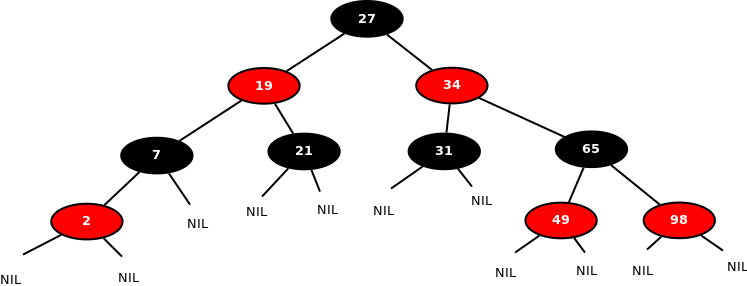
\includegraphics[width=\textwidth]{images/rb_tree.png}
\caption{Piros fekete fa a processz prioritás értékekkel}
\label{fig:rb_tree}
\end{figure}
\SubSection{Kernel modul}
%TODO The Linux Kernel Module Programming Guide. Peter Jay Salzman Michael Burian Ori Pomerantz. Copyright © 2001 Peter Jay Salzman.  
%TODO Understanding the Linux Kernel, Third Edition by Daniel P. Bovet and Marco Cesati
Egy modul gyakorlatilag instrukciók sorozata, amit igény szerint, ki és be lehet tölteni a kernel-be. Kibővíti a kernel funkcionalitását, anélkül hogy újra keljen indítani a rendszert. Minden magasabb szintű kernel komponens, mint például fájlrendszerek, I/O eszköz driver, hálózati rétegek, stb, meg lehet írni modulként és be lehet tölteni a kernel-be.

\noindent Az éppen aktuálisan betöltött moduljainkat, le tudjuk kérdezni az \texttt{\# lsmod} paranccsal, ami a \texttt{/proc/modules} fájl tartalmát listázza.

A modulok ELF objektumként tárolódnak a fájlrendszeren, amik a kernelhez vannak linkelve, ezt a linkelést az \texttt{\# insmod} paranccsal tudjuk elvégezni.
A modulok egy duplán láncolt listában tárolódnak.
Ha ebből a listából el szeretnénk távolítani egy modult(unlink), az \texttt{\# rmmod} programot használhatjuk, ami a következő műveleteket végzi el:
\begin{enumerate}
	\item Beolvassa a parancssorból annak a modulnak a nevét, amit el kívánunk távolítani.
	\item Megnyitja a \texttt{/proc/modules} fájlt és leellenőrzi hogy a modul, ténylegesen linkelve van-e a listába.
	\item Meghívja a \texttt{delete\_modul()} rendszerhívást és továbbadja neki a modul nevét.
	\item Terminálódik.
\end{enumerate} 

Minden kernel modulnak kell hogy legyen legalább két eljárása, az egyik ilyen \texttt{init\_module()}.
Ez egy inicializációs eljárás, az \texttt{init\_module()} hívódik meg amikor beszúrjuk a modult az \texttt{insmod} paranccsal.
A másik a \texttt{cleanup\_module()}, ami pedig az eltávolítás során(\texttt{rmmod}) hívódik meg.
A 2.3.13.-as kernel verzióban bevezettek egy újítást, ami szerint, mi határozhatjuk meg az eljárások neveit. Ehhez használjuk a \texttt{module\_init()} és a \texttt{module\_exit()} makrókat. Tipikusan, az \texttt{init\_module()}-ban írjuk meg a programunkat, ami lehet hogy kicserél egy kernel függvényt a miénkre vagy regisztrál valamilyen kezelőt a kernel-hez. A \texttt{cleanup\_module()}-nak pedig az lenne a feladata, hogy visszavonja a módosításokat, amit az \texttt{init\_module()} elvégzett.
%https://www.kernel.org/doc/htmldocs/kernel-hacking/routines-init-again.html

A prink() függvénynek, nem a felhasználóval történő kommunikáció a fő szerepe, mégha én a mostani példában arra is használom. Ez egy naplózási eszköz(log) a kernel számára, amivel valamilyen fontos információt vagy hibaüzenetet továbbít. Az üzeneteknek, különböző fontossági szintjük van. Ezeket a szinteket hívjuk console\_loglevel-nek, ami egy kernelbeli változó, aminek a szintjeit 0-7 ig fogjuk megnézni. 
%https://www.kernel.org/doc/html/latest/core-api/printk-basics.html
\begin{enumerate}
\setcounter{enumi}{-1}
	\item KERN\_EMERG \- Ezen a log-szinten, a rendszerünk már használhatatlan állapotba került.
	\item KERN\_ALERT \- Az adódott problémákról, gondoskodnunk kell.
	\item KERN\_CRIT \- Kritikus események jelentkeztek.
	\item KERN\_ERR \- Nem kritikus hibák jelzése.
	\item KERN\_WARNING	\- Figyelmeztetések, amikre oda kell figyeljünk.
	\item KERN\_NOTICE \- Normális, általános események
	\item KERN\_INFO \- Információ továbbítás ami nem igényel beavatkozást.
	\item KERN\_DEBUG \- Kernelbeli hibakiíratás, egy kimenet a kernel oldalról, hogyha a fejlesztő bekapcsolta a \texttt{debugging at compile time}-ot.
\end{enumerate}
Az aktuális console\_loglevel-t, meg tudjuk jeleníteni futásidőben, a következő paranccsal:
\begin{cpp}
$ cat /proc/sys/kernel/printk 
4        4        1        7
\end{cpp}
%$
Ezek a számok, az aktuális, alapértelmezett, minimális és boot-time-default log szinteket mutatják.

A cél nálam az ütemező optimalizálása volt, különféle operációs rendszer felhasználati módok esetében. Emiatt szükségem volt az éppen aktuális processzek adataira.
Ehhez a feladathoz készítettem egy betölthető modult, amiben a \texttt{printk()}-függvényt használtam, a processz adatok naplózására.
A processzek az operációs rendszeren belül, egy duplán láncolt listában helyezkednek el.
A processzek végigjárásához létezik egy \texttt{for\_each\_process} makró.
\begin{cpp}
struct task_struct *p;
#define for_each_process(p) \
	 for ( p = &init_task ; ( p = next_task(p)) != &init_task ; )
\end{cpp}
Ennel felhasználásával könnyen végig tudtam iterálni, a rendszerben lévő processzeken. A szükséges adatokat a processzekről, az őket definiáló struktúra váltózóiként értem el. Ez struktúra a \texttt{/linux/sched.h}-ban található.
\begin{cpp}
 printk(KERN_INFO "/comm/and: \%s pid: \%d 
 prio: \%d rt_prio: \%d weight: \%lu 
 vruntime: \%llu pcount:\%lu 
 \\nsum_exec_runtime:\%llu 
 prev_sum_exec_runtime:\%llu 
 exec_start:\%llu\\n",p->comm,p->pid, 
 p->prio,rt_task(p),p->se.load.weight,p->se.vruntime,
 p->sched_info.pcount,p->se.sum_exec_runtime,
 p->se.prev_sum_exec_runtime,p->se.exec_start);
\end{cpp}


%TODO https://doc.opensuse.org/documentation/leap/archive/42.1/tuning/html/book.sle.tuning/cha.tuning.taskscheduler.html
\SubSection{Ütemezési politikák(Scheduling policy)}
A linux kernel a következő ütemezési politikákat támogatja:
\begin{itemize}
    \item SCHED\_FIFO - Időkritikus valós idejű processzek ütemezésére használják. Az elsőnek érzekett processz kerül először kiszolgálásra.

	\item	SCHED\_RR - SCHED\_FIFO-hez hasonló, szintén valós idejű processzekhez használják. A Kerge Rigó ütemezési algoritmust használja.

    \item SCHED\_BATCH - CPU lázas processzek ütemezésére tervezték.
    
	\item SCHED\_IDLE - Ezt az ütemezési politikát, kis intenzitású processzek esetén használják
	
	\item SCHED\_OTHER - Alapértelmezett ütemezési algoritmus, amit a normál processzek nagytöbbsége is használ.

\end{itemize}

\SubSection{Processz Prioritási szintek és azok módosítása}
\begin{cpp}
struct task_struct {
...	
		int				prio;
...
};
\end{cpp}

A \texttt{prio} paramétert az adott processz, prioritási szintjének meghatározására, használja az ütemező. Egy processz statikus prioritási értéke, pedig adott ütemezési politikákhoz mérten változhat. Ezeket a \texttt{chrt -m} paranccsal láthatjuk.
\begin{cpp}
$ chrt -m
SCHED_OTHER min/max priority	: 0/0
SCHED_FIFO min/max priority	: 1/99
SCHED_RR min/max priority	: 1/99
SCHED_BATCH min/max priority	: 0/0
SCHED_IDLE min/max priority	: 0/0
SCHED_DEADLINE min/max priority	: 0/0
\end{cpp}
%$
Normál processzek esetén 120-as a statikus prioritás, ezt az értéket módosíthatjuk, a nice illetve a renice-paranccsal.
Ez a nice érték -20 és +19 között mozoghat, attól függően hogy mennyire szeretnénk nagylelkűek lenni, a többi processzel szemben.
A 100 prioritási szint, a legfontosabb amíg a 139-es a legkevésbé fontos.
Egy átlagos taskból is készíthetünk realtime processzt, ekkor viszont másik runqueue-ba( \texttt{rt\_rq} ) kerül és egy másik ütemező fog velük foglalkozni. Real time processzek készítésénél, megválaszthatjuk hogy RR(Kerge Rigó) vagy FIFO(First in, First out) ütemező algoritmust szeretnénk. 

chrt - <ütemező algoritmus> <prioritási szám> <futtatható program vagy -p pid>
program segítségével készíhetünk valós idejű processzeket.
RealTime processzek esetén, a prioritási szintek megfordulnak, a legnagyobb szám jelzi a legfontosabb processz prioritási szintet.
99-es prioritás jelzi a legfontosabb processzt és 0-ás a legkevésbé fontosat.

%TODO Benchmarkok(phoronix)
%TODO https://www.phoronix-test-suite.com/
\SubSection{Benchmark}
Az ütemező optimalizálására végzett különböző módosításaim, megjelenítésére a Phoronix Test Suite (PTS) programot használom.
A Phoronix Test Suite a rendelkezésre álló legátfogóbb tesztelési és benchmarking platform, amely kibővíthető keretet biztosít, azaz új tesztek is egyszerűen hozzáadhatók.
A szoftvert úgy tervezték hogy, mind kvalitatív, mind kvantitatív benchmark méréseket lehessen végezni, egyszerűen, hatékonyan és reprodukálhatóan.
  
%TODO Adott benchmarkok bemutatűsa
Processzor igényes benchmarkokhoz, több félét is választottam. Az első, a Sample Pi Program volt, a benchmark egy \texttt{C++} nyelven írt program, ami a Pi-t, a 8,765,4321 számjegyéig kiszámolja Leibniz formula alapján. Ez egyetlen processzként próbálja megterhelni, valamelyik processzor magot.

A második processzor igényes program, az ebizzy tesztje. Ez egy olyan program amely egy webszerver munkaterheléséhez hasonló processzeket generál. Az előzővel ellentétben, ez már egyszerre több processzben indul el és fut le. Emiatt itt mégnagyobb szerepet kap az ütemező és az optimalizálási kisérleteim bemutatására szánt statégiáim.
 
%TODO Adott probléma megközelítési módjai

%TODO Prio 
%TODO Sysctl interface -> kernel.sched_*(paraméterek)
%TODO Sysctl kernel.sched 
%TODO Script program leírása, bemutatása

